\documentclass[border=5mm]{standalone}
\usepackage{tikz}
\usepackage{amsmath, amssymb}\usetikzlibrary{positioning}
\usepackage{graphicx}
\usetikzlibrary{positioning,calc,arrows.meta,shapes.geometric}

\begin{document}
% Narrow layout for responsive rendering: the macro sequence flows down into
% h_t, firm characteristics enter from the left, and the combined state then
% continues vertically through the feed-forward network to the SDF weights.
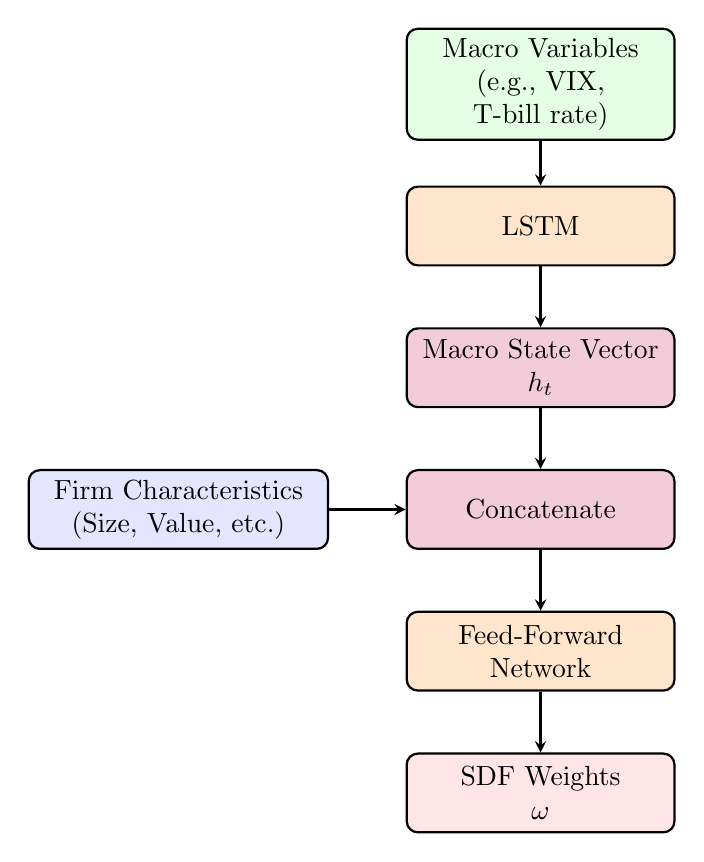
\begin{tikzpicture}[
        node/.style={draw, rectangle, rounded corners, minimum width=3.4cm, minimum height=1cm, text width=3.0cm, align=center, thick},
        arrow/.style={-stealth, thick}
    ]
        % Macro side
        \node[node, fill=green!10] (macro) at (2.3, 8.6) {Macro Variables\\(e.g., VIX, T-bill rate)};
        \node[node, fill=orange!20] (lstm) at (2.3, 6.8) {LSTM};
        \node[node, fill=purple!20] (state) at (2.3, 5.0) {Macro State Vector\\$h_t$};

        % Firm characteristics side
        \node[node, fill=blue!10, minimum width=3.8cm, text width=3.4cm] (chars) at (-2.3, 3.2) {Firm Characteristics\\(Size, Value, etc.)};

        % Concatenation and FFN
        \node[node, fill=purple!20] (concat) at (2.3, 3.2) {Concatenate};
        \node[node, fill=orange!20] (ffn) at (2.3, 1.4) {Feed-Forward\\Network};
        \node[node, fill=red!10] (output) at (2.3, -0.4) {SDF Weights\\$\omega$};

        \draw[arrow] (macro) -- (lstm);
        \draw[arrow] (lstm) -- (state);
        \draw[arrow] (state) -- (concat);
        \draw[arrow] (chars) -- (concat);
        \draw[arrow] (concat) -- (ffn);
        \draw[arrow] (ffn) -- (output);
    \end{tikzpicture}

\end{document}
